\section{Study of the CP properties of the top-quark Yukawa interaction in t\bar{t}H and tH events wth H \rightarrow \gamma \gamma: Categorization} \label{sec:ttHCPCategorization}

In order to properly measure the dependence of the top Yukawa coupling on the CP-mixing angle $\alpha$, we divide a region of $ttH$-and-$tH$-enriched phase space into a number of different categories based both upon the similarity of events it contains to signal (Higgs processes like $ttH$ and $tH$) rather than background (non-Higgs continuum diphoton processes), as well as the similarity of events it contains to CP-odd rather than CP-even Higgs processes. By creating many such categories and fitting the event yield in each, we can set detailed constraints on the value of $\alpha$.

First, we define two sets of regions. The "hadronic" region targets events containing fully-hadronic top decays, requiring two loose-ID photons, one b-tagged jet at the 77\% working point with $p_{T} > 25$ GeV, as well as two additional jets with $p_{T} > 25$ GeV and exactly zero electrons or muons. Similarly, the "leptonic" region targets events containing semi-leptonic top decays, requiring two loose-ID photons, one b-tagged jet at the 77\% working point with $p_{T} > 25$ GeV, as well as at least one isolated electron or muon.

To perform the categorization in these regions, two multivariate Boosted Decision Trees (BDTs) are used, one to separate Higgs events from background and one to separate CP-odd Higgs events from CP-even Higgs events. Both BDTs are trained on low-level kinematic features using the XGBoost package \ref{cite:XGBoost}. We then define a series of cuts on these BDT scores, defining a total of 20 orthogonal regions, each with differing sensitivity both to the $ttH+tH$ signal and to the CP-odd $ttH+tH$ hypothesis.

\subsection{SBBDT}

The signal-versus-background BDT (SBBDT) developed for use in the CP Analysis is identical to that developed first in the $79.8 fb^{-1}$ measurements of $ttH$ in the diphoton channel \ref{cite:HIGG-2018-13} in and later retrained for $139 fb^{-1}$ measurements of $ttH$ in the diphoton channel \ref{cite:ATLAS-CONF-2019-004}. It is trained separately for both the hadronic and leptonic regions.

Both the hadronic and leptonic BDTs are trained using a Standard-Model Powheg $ttH$ Monte Carlo sample to model the signal and NTI data control events to model the continuum diphoton background.

\subsubsection{Hadronic Region} \label{sec:SBBDThad} 
In the hadronic region, 60\% of the $ttH$ Monte Carlo signal events are used for training, 20\% are reserved for categorization and BDT hyperparameter optimization, and the final 20\% are reserved for validation. 60\% of the NTI events are used for training, 20\% are reserved for hyperparameter optimization, and the remaining 20\% are reserved for testing and significance evaluation.

The input variables chosen are: 

\begin{itemize}
\item $p_T/m_{\gamma \gamma}$, $\eta$ and $\phi$ of the two photons. Photon $p_{T}$ is scaled by $m_{\gamma \gamma}$ to reduce unwanted sculpting of the diphoton mass spectrum. 
\item $p_T$, $\eta$, $\phi$ and E of the six jets with highest $p_{T}$
\item Boolean b-tag flag (77\% working point) for each of the six jets with highest $p_{T}$
\item \MET and direction of \MET
\end{itemize}

Distributions of the BDT input variables using $79.8 fb^{-1}$ of data are shown in Figure \ref{fig:SBBDTvarshad}.

\begin{figure}
	\centering
	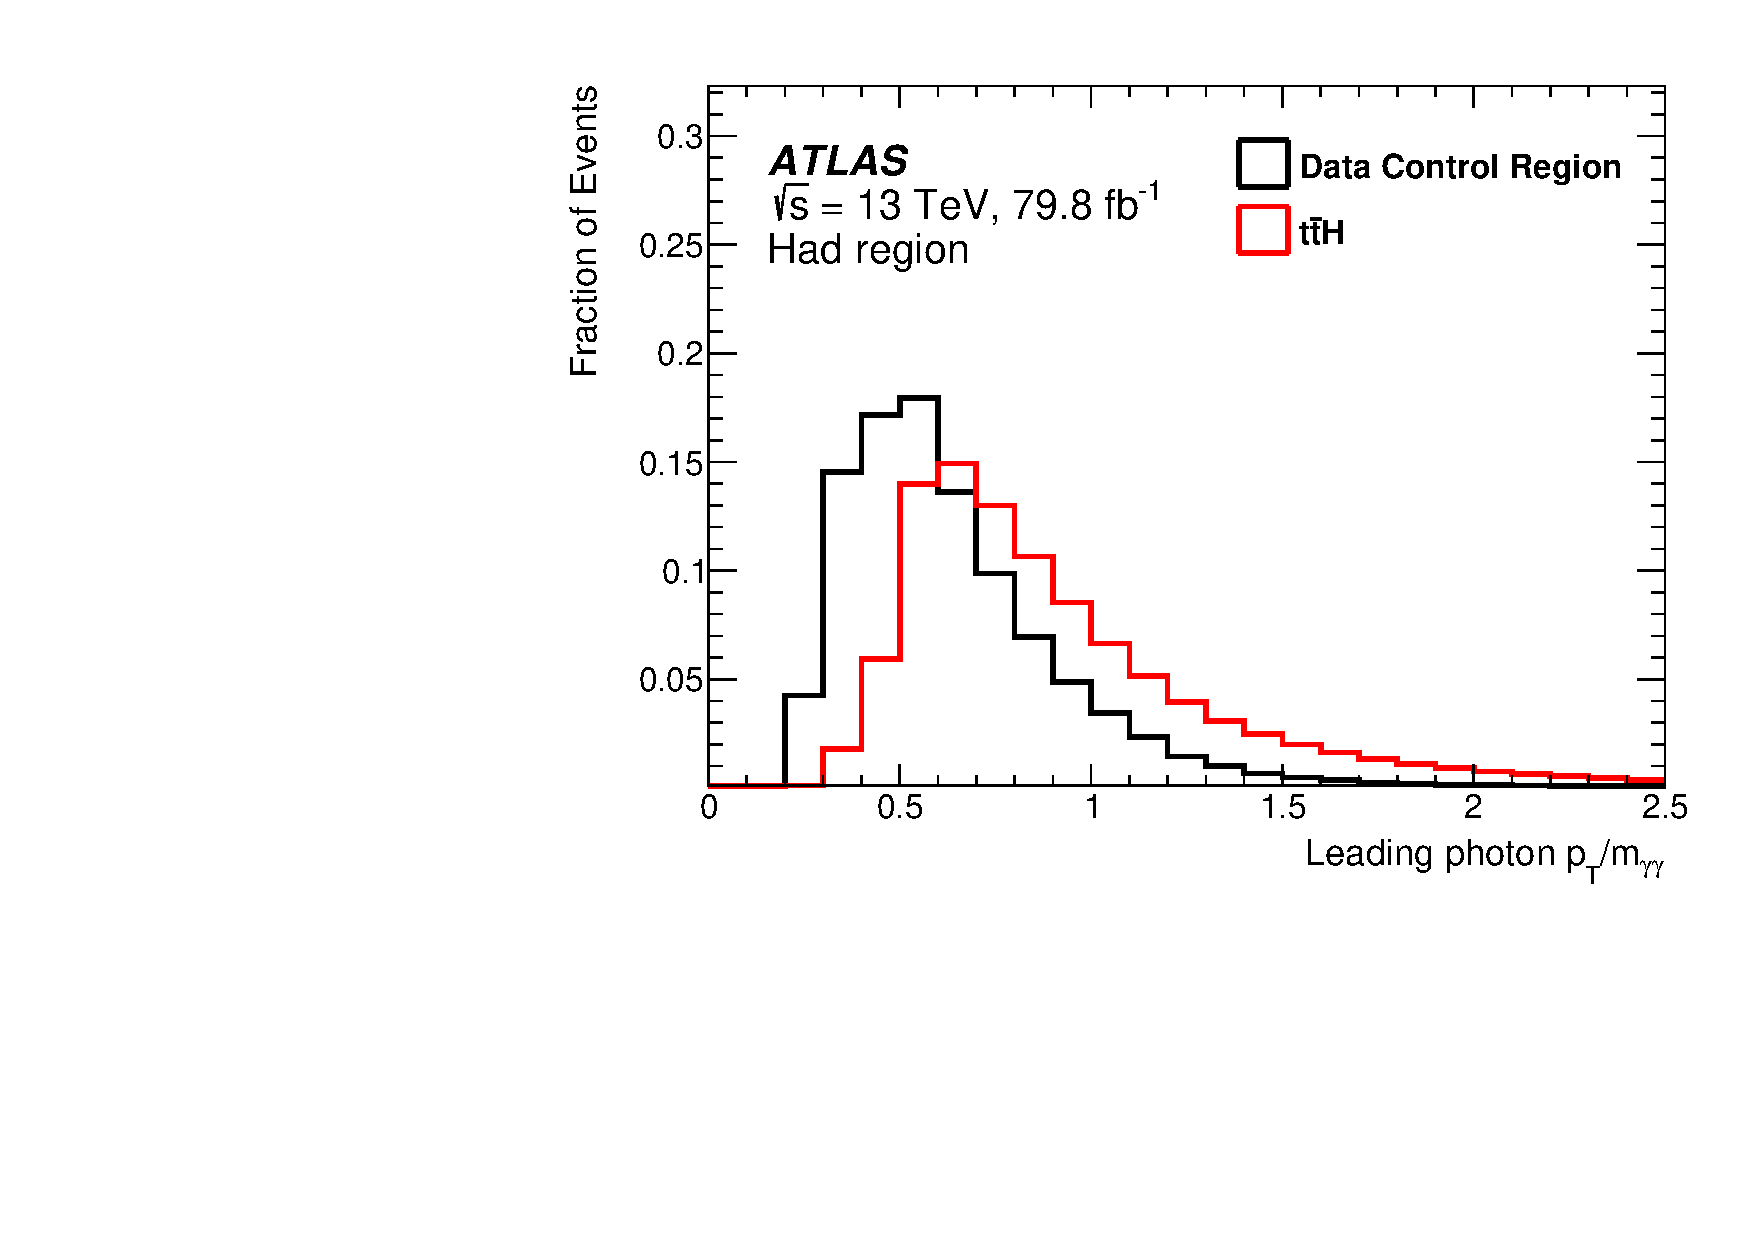
\includegraphics[width=0.31\linewidth]{figures/tthcp_chapter/figaux_10a.pdf}
	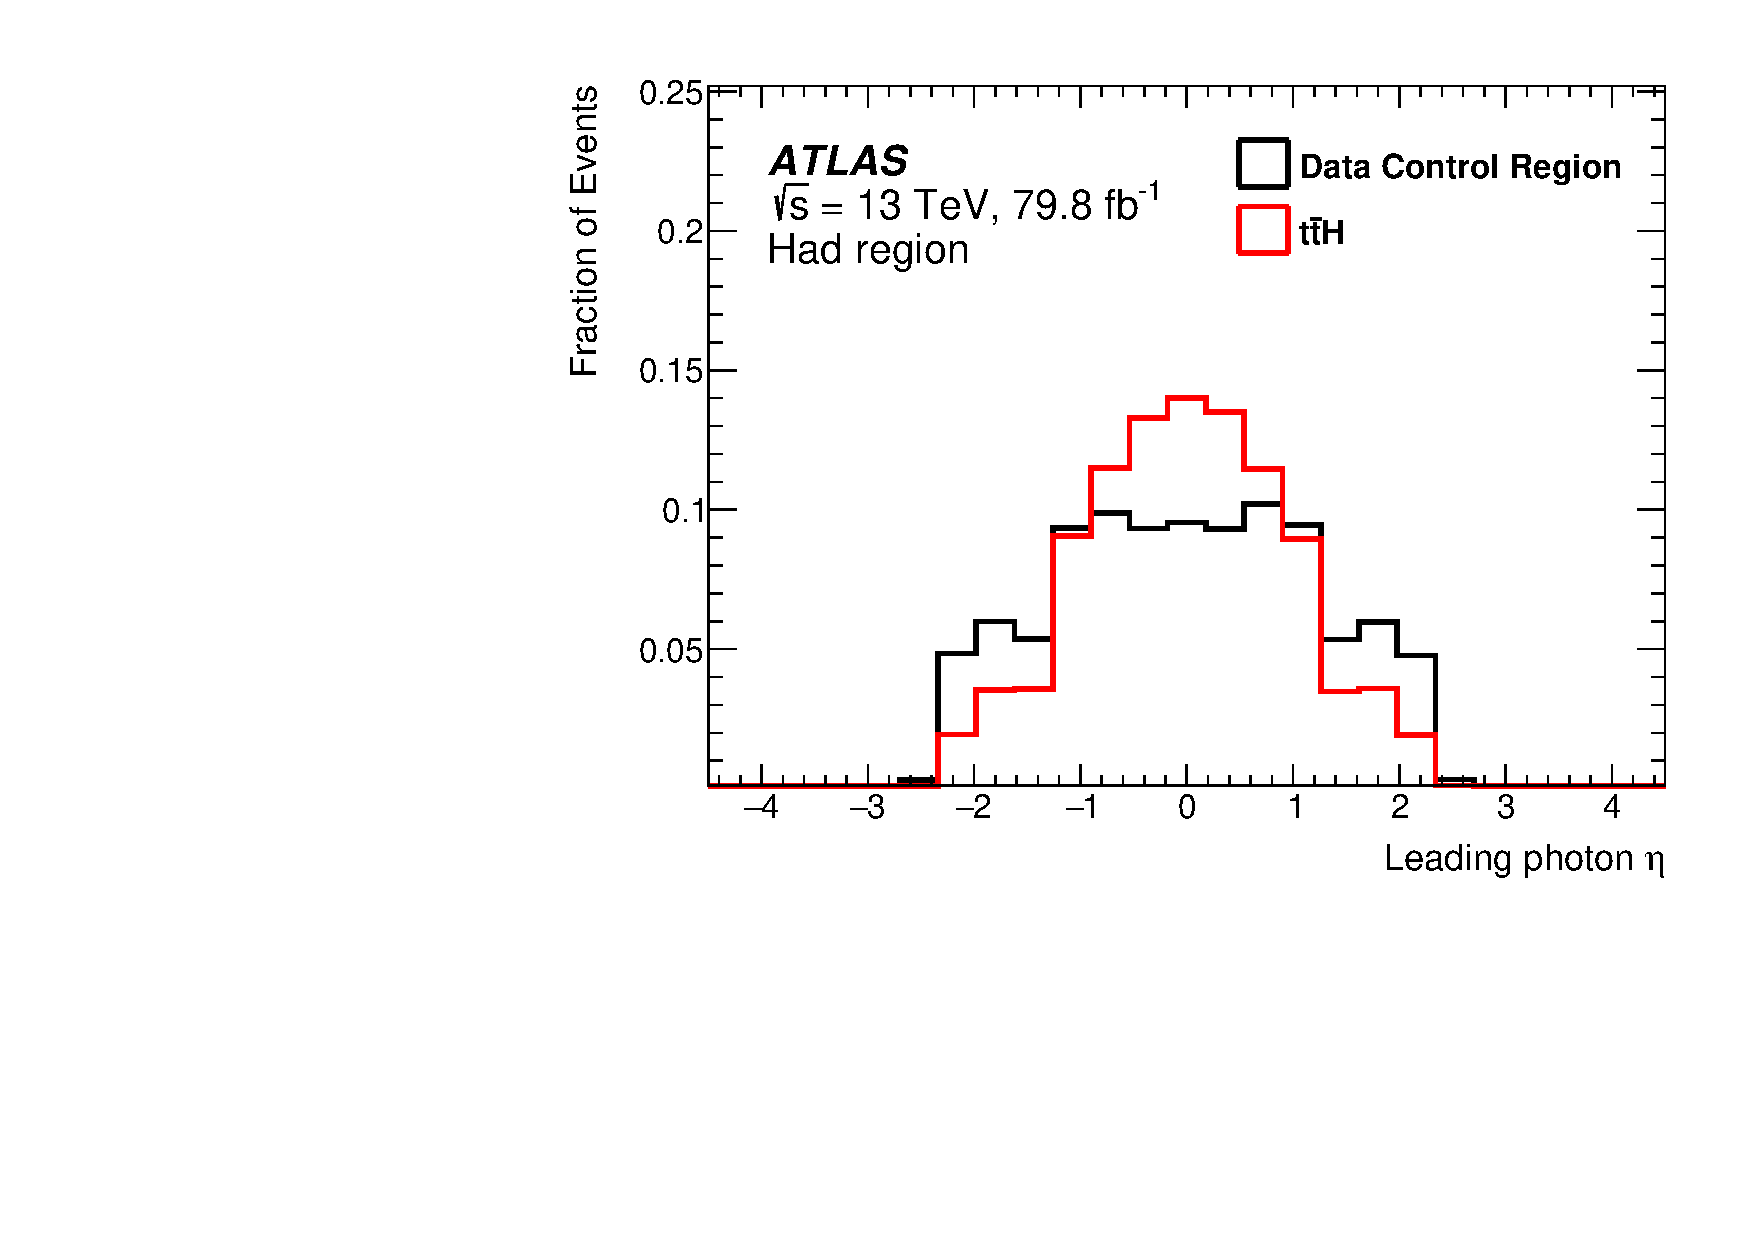
\includegraphics[width=0.31\linewidth]{figures/tthcp_chapter/figaux_10b.pdf}
	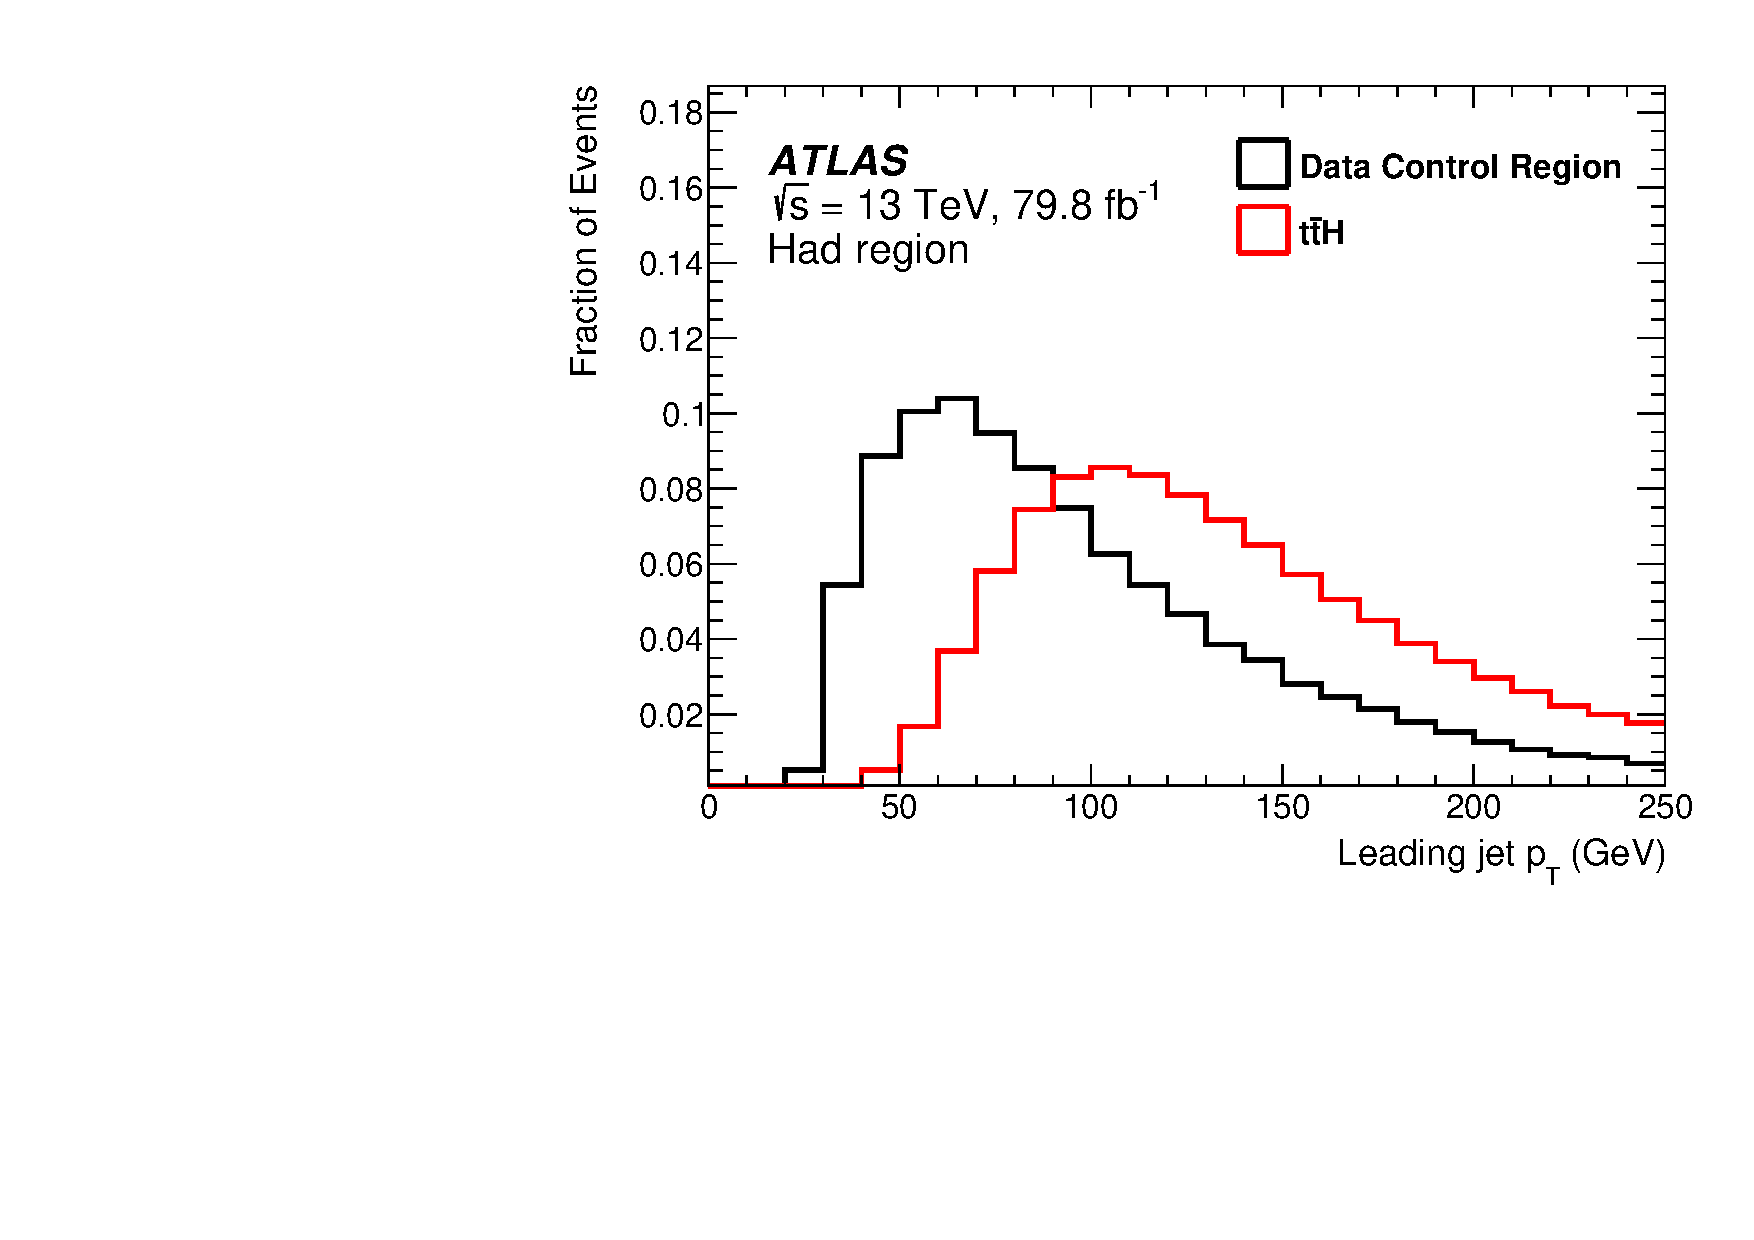
\includegraphics[width=0.31\linewidth]{figures/tthcp_chapter/figaux_10c.pdf}
	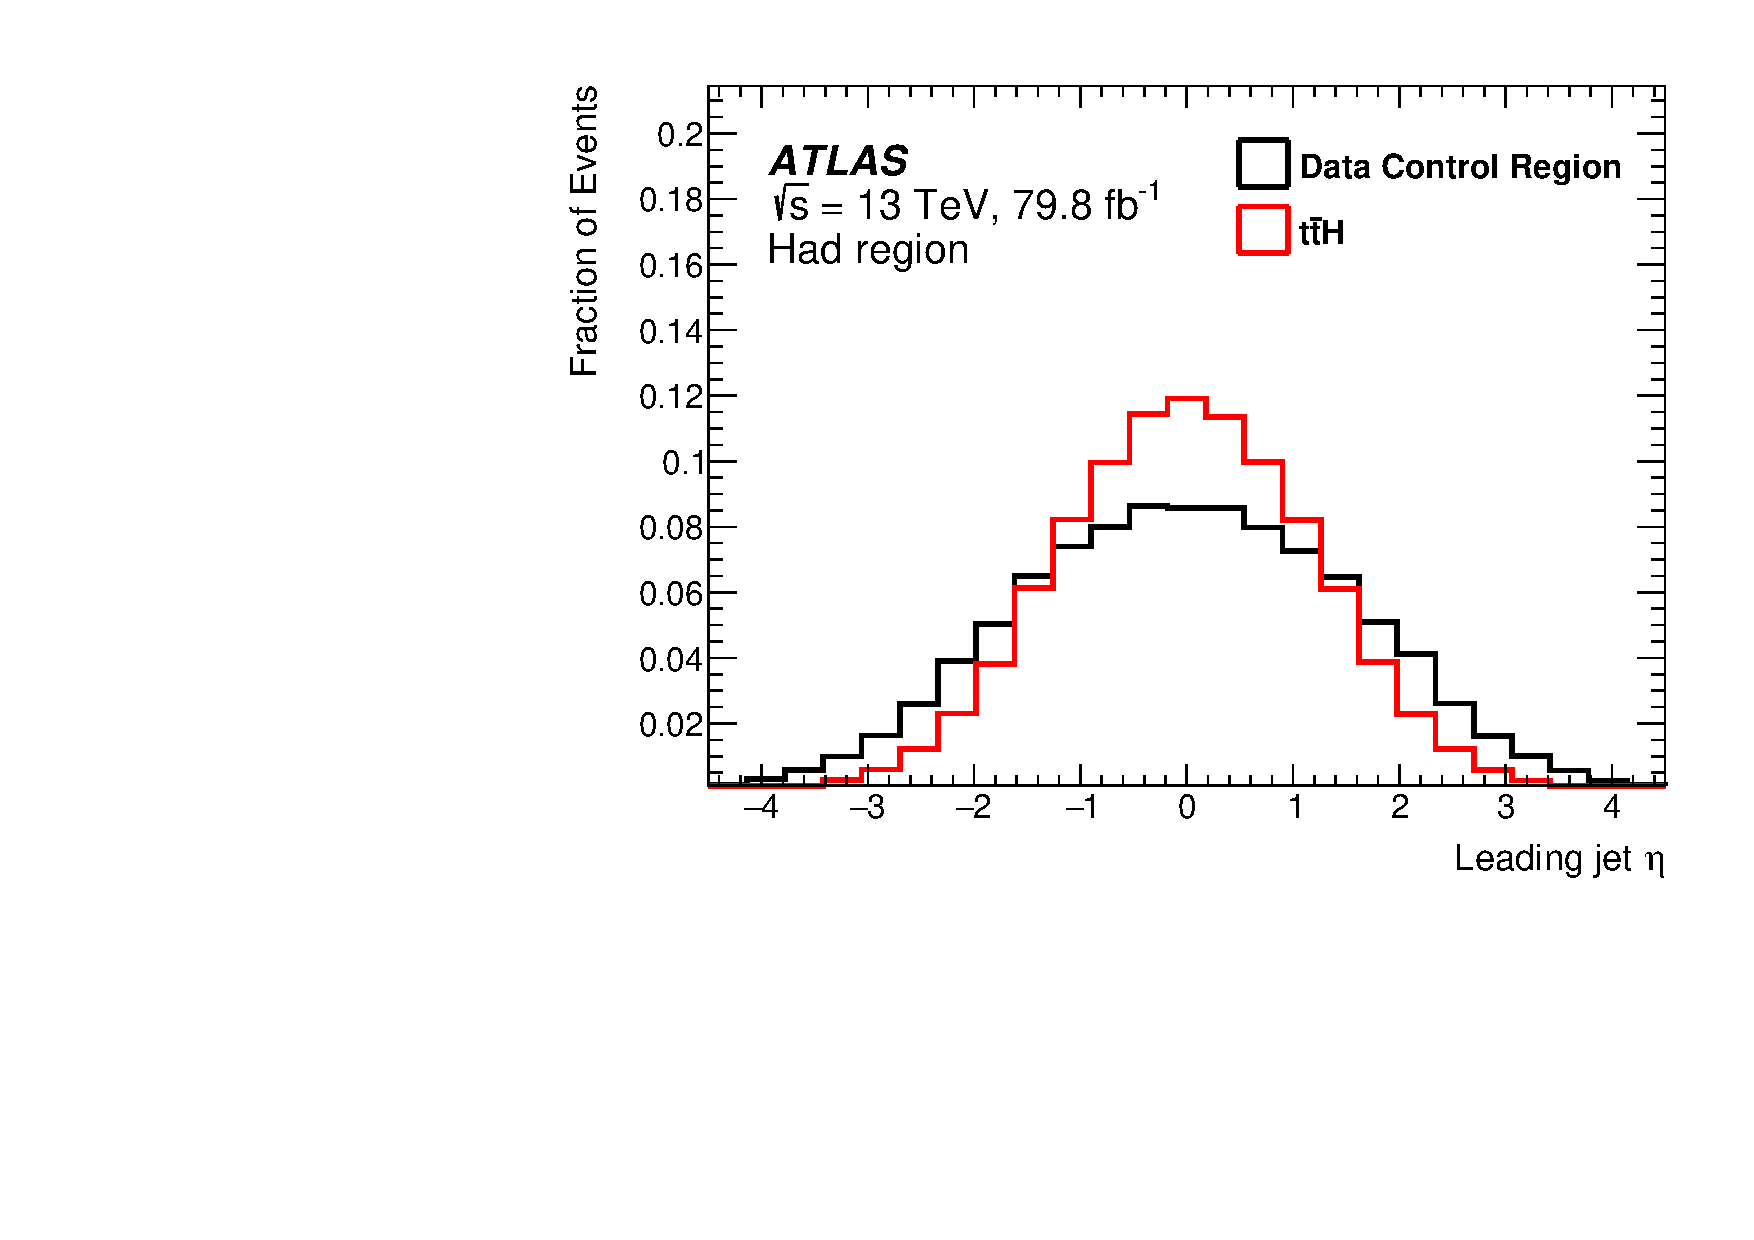
\includegraphics[width=0.31\linewidth]{figures/tthcp_chapter/figaux_10d.pdf}
	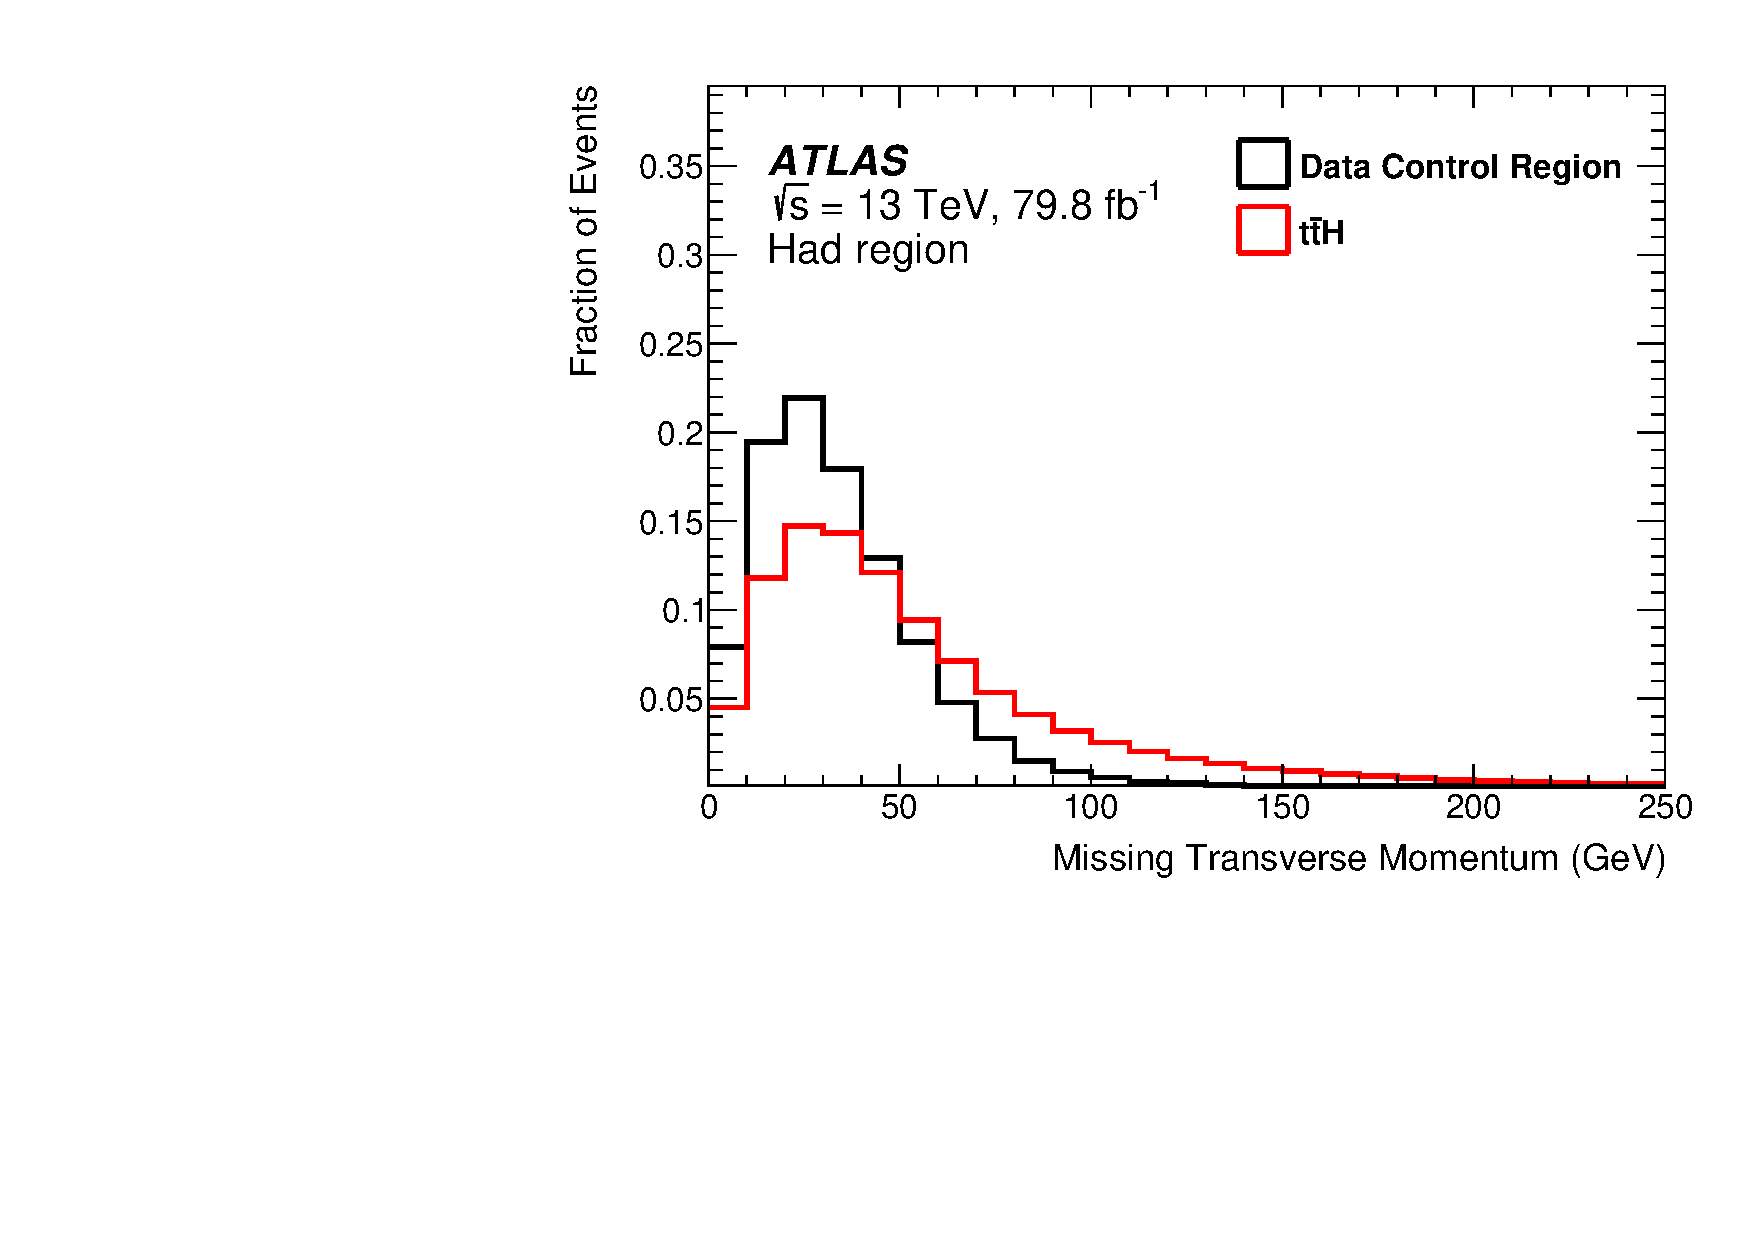
\includegraphics[width=0.31\linewidth]{figures/tthcp_chapter/figaux_10e.pdf}
	\caption{Distributions of training variables for the hadronic background-rejection BDT, trained at 79.8 fb^{-1}. Taken from \ref{cite:HIGG-2018-13}. }
	\label{fig:SBBDTvarshad}
\end{figure}

\subsubsection{Leptonic Region} \label{sec:SBBDTlep} 

As in the hadronic region, in the leptonic region, 60\% of the $ttH$ Monte Carlo signal events are used for training, 20\% are reserved for categorization and BDT hyperparameter optimization, and the final 20\% are reserved for validation. 75\% of the NTI events containing zero b-jets but at least one un-tagged jet wiare used for training and the remaining 25\% are reserved for hyperparameter optimization, while 50\% of the NTI events containing one or more b-jets are used for categorization and the remaining 50\% are reserved for testing and significance evaluation.

However, due to lower statistics in the leptonic top decay channel due to the smaller top-quark branching ratio to leptons, two cuts are relaxed for the development of the leptonic BDT:

\begin{itemize}
\item The relative $p_{T}$ cuts are loosened from $\frac{p_{T}}{m_{\gamma\gamma} > 0.35$ for the leading photon and $\frac{p_{T}}{m_{\gamma\gamma} > 0.25$ for the subleading photon to a flat $p_{T} > 35$ GeV for the leading photon and $p_{T} > 25$ GeV for the subleading photon.
\item The diphoton invariant mass window is extended from $105 GeV < m_{\gamma \gamma} < 160 GeV$ to $80 GeV < m_{\gamma \gamma} < 250 GeV$.
\end{itemize}

The cuts are again tightened to define the signal region after BDT training is complete- that is, the loosening of these cuts is only utilized to increase BDT training statistics, and does not carry through to other stages of the analysis.

The input variables chosen are: 

\begin{itemize}
\item $p_T/m_{\gamma \gamma}$, $\eta$ and $\phi$ of the two photons. Photon $p_{T}$ is scaled by $m_{\gamma \gamma}$ to reduce unwanted sculpting of the diphoton mass spectrum.
\item $p_T$, $\eta$ and $\phi$ of up to two leptons. 
\item $p_T$, $\eta$, $\phi$ and E of the four jets with highest $p_{T}$
\item Boolean b-tag flag (77\% working point) for each of the four jets with highest $p_{T}$
\item \MET and direction of \MET
\end{itemize}

Distributions of the BDT input variables using $79.8 fb^{-1}$ of data are shown in Figure \ref{fig:SBBDTvarslep}. The BDT output distributions are shown in figures \ref{fig:moriondtotal}. We note that the SBBDT performance is independent of $\alpha$.

\begin{figure}
	\centering
	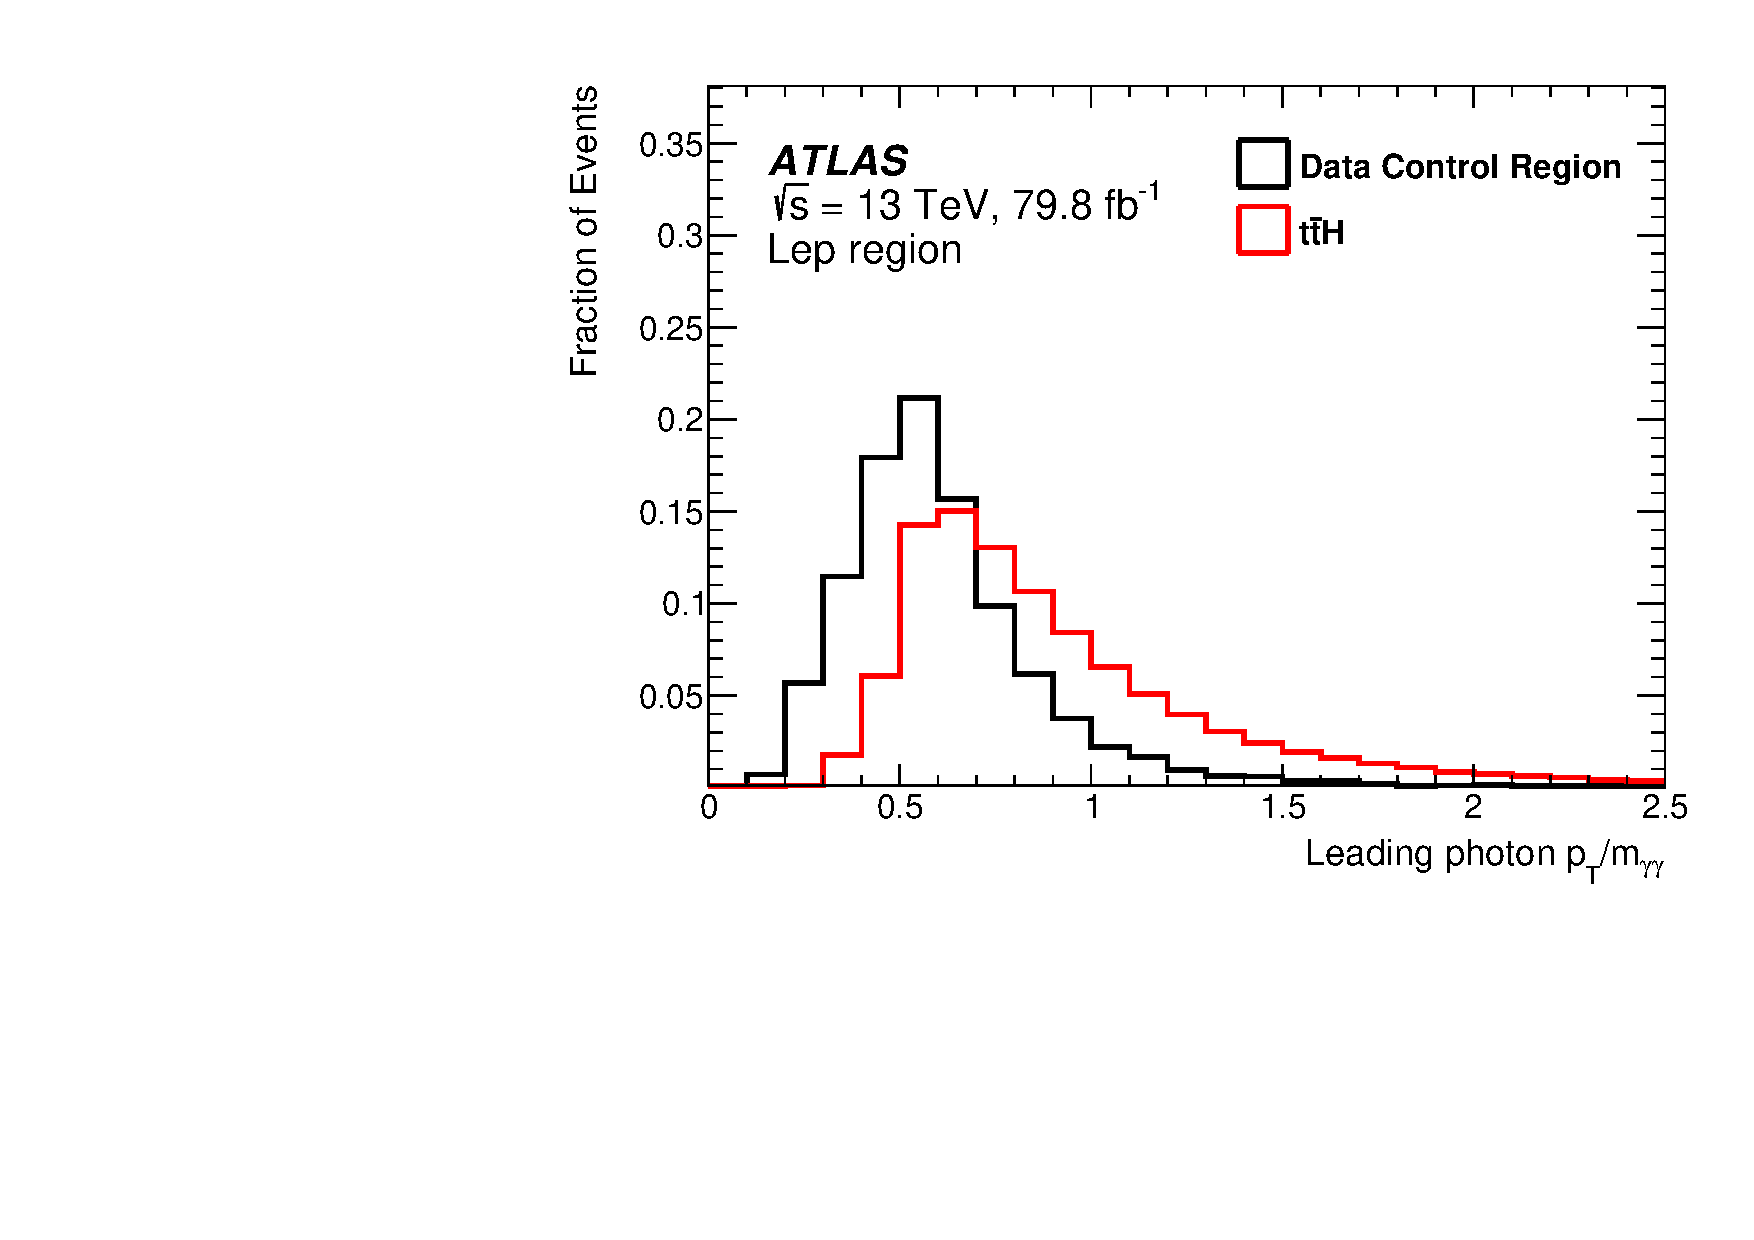
\includegraphics[width=0.31\linewidth]{figures/tthcp_chapter/figaux_11a.pdf}
	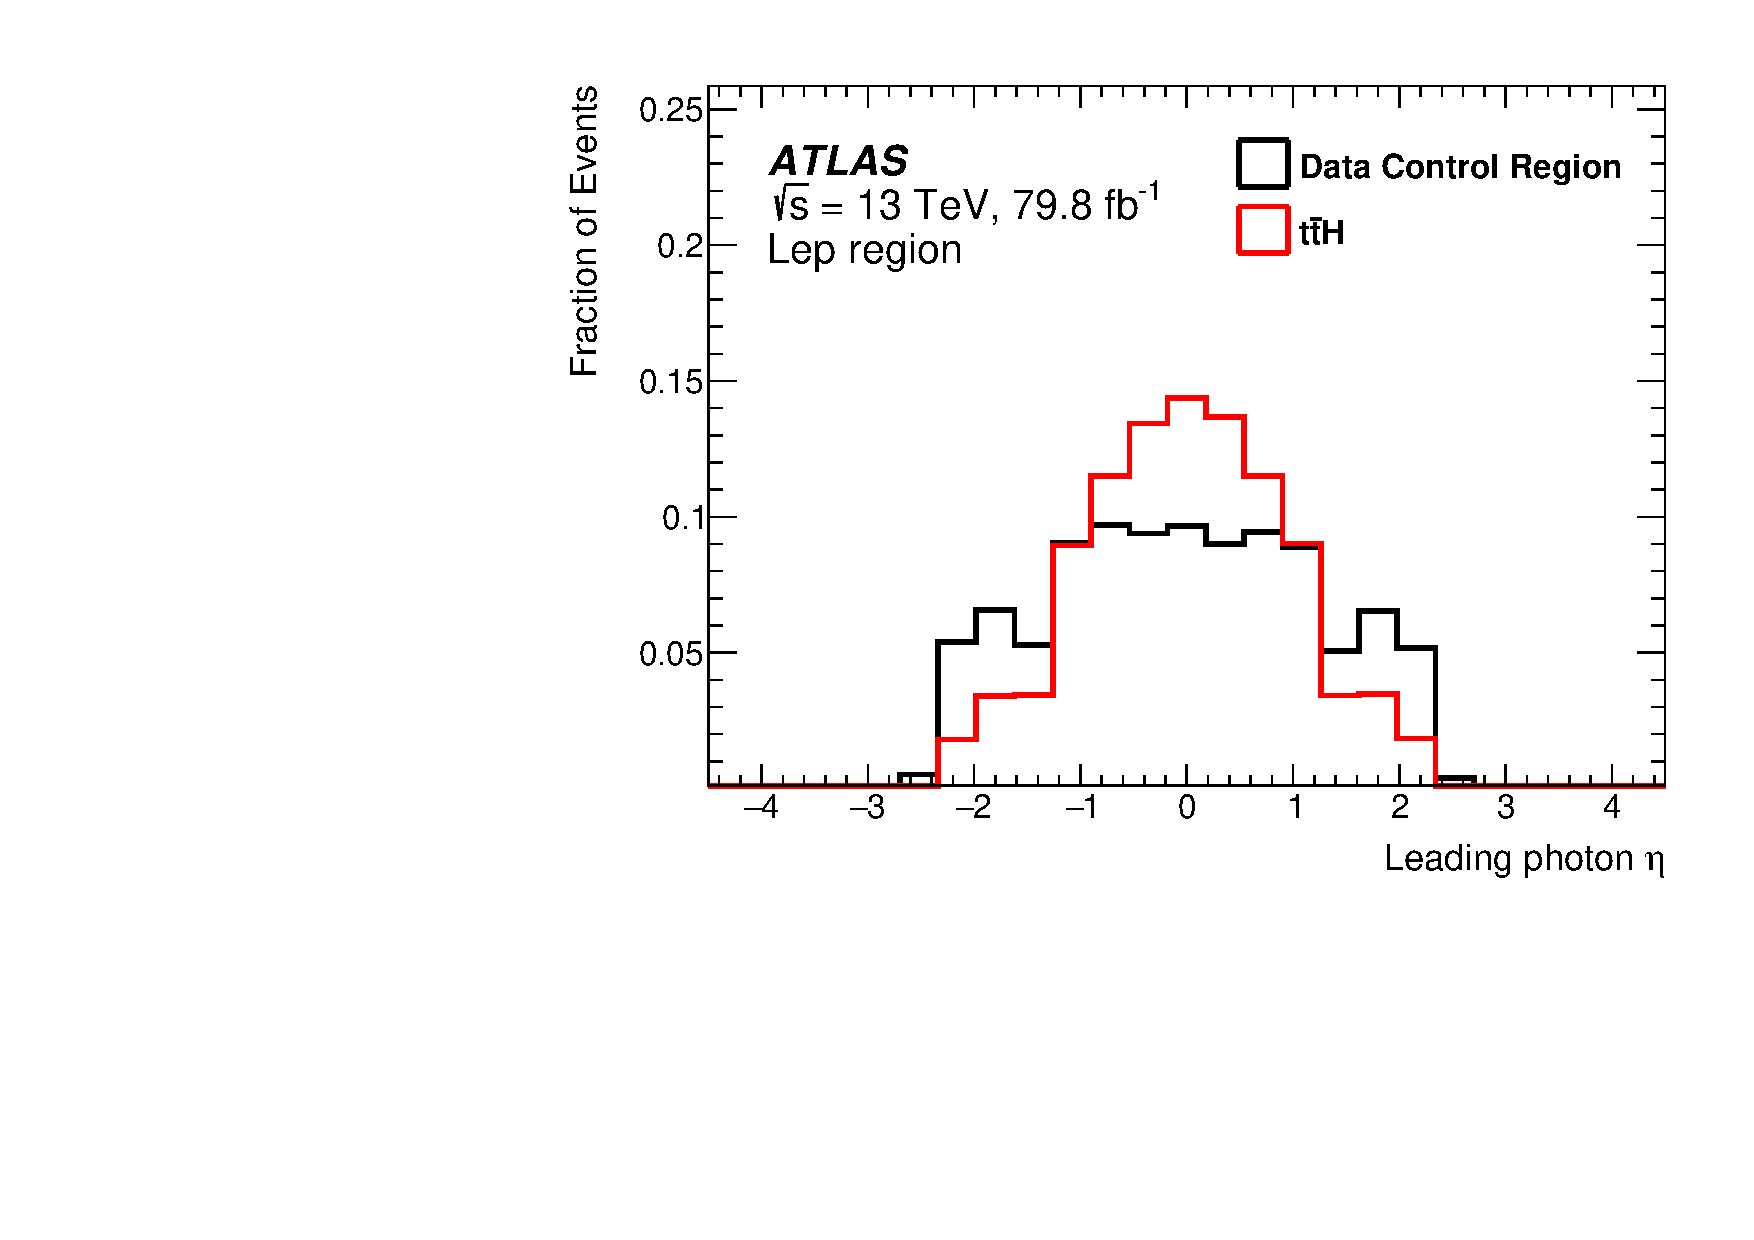
\includegraphics[width=0.31\linewidth]{figures/tthcp_chapter/figaux_11b.pdf}
	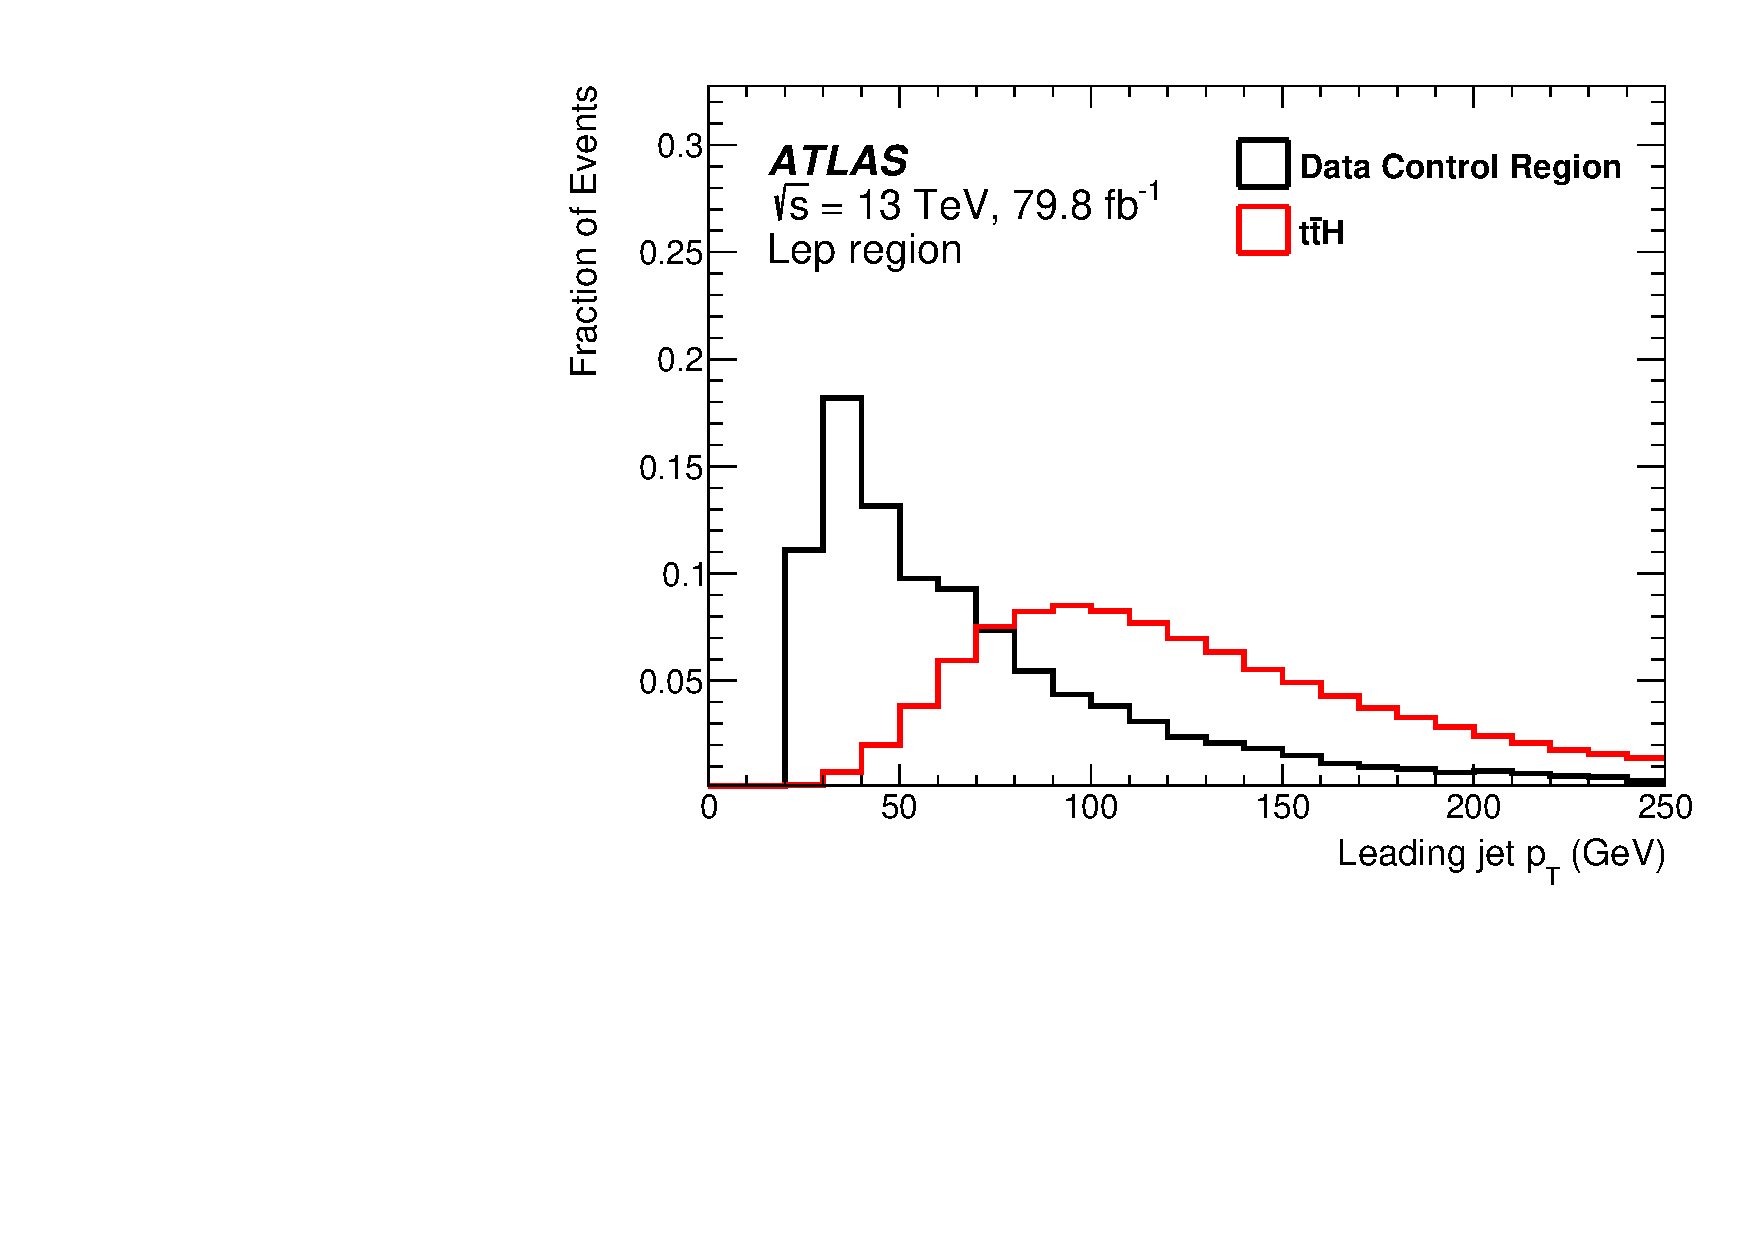
\includegraphics[width=0.31\linewidth]{figures/tthcp_chapter/figaux_11c.pdf}
	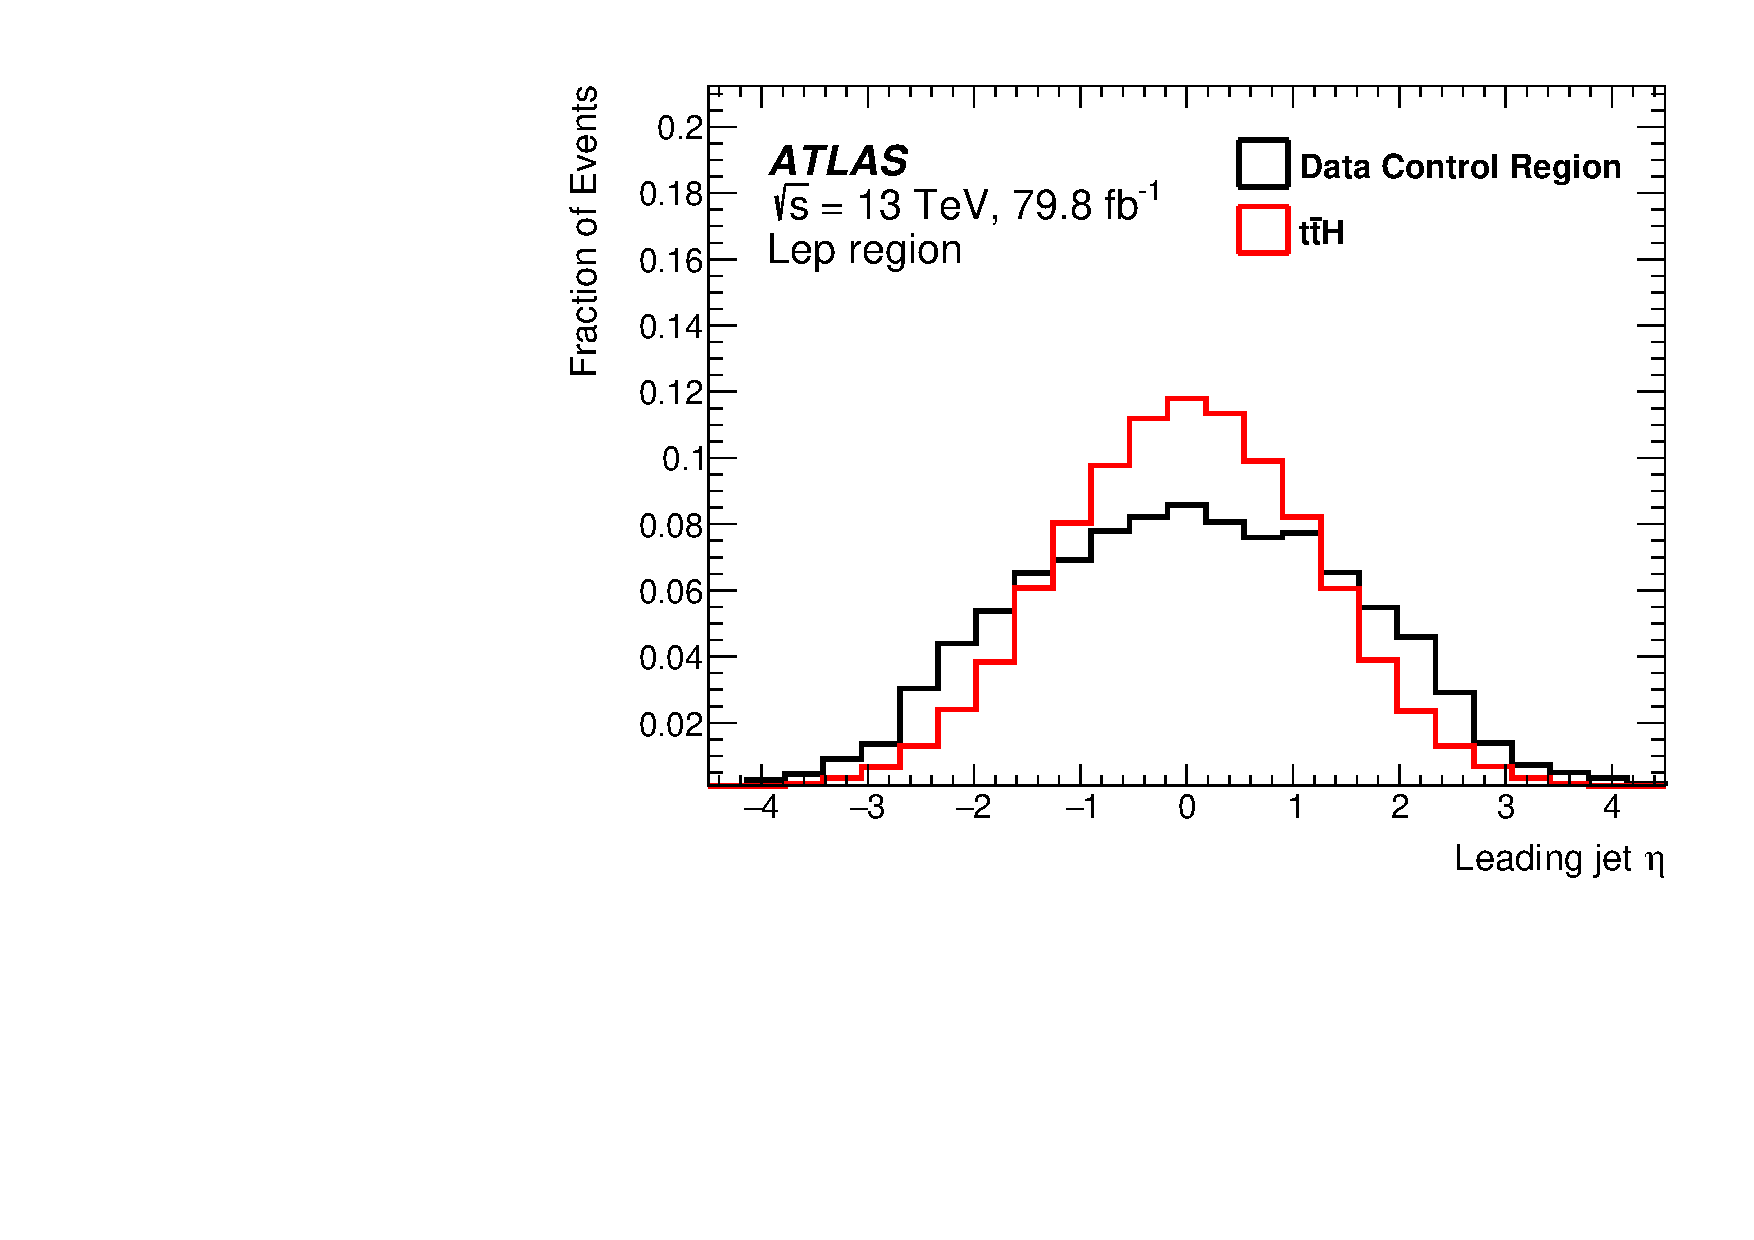
\includegraphics[width=0.31\linewidth]{figures/tthcp_chapter/figaux_11d.pdf}
	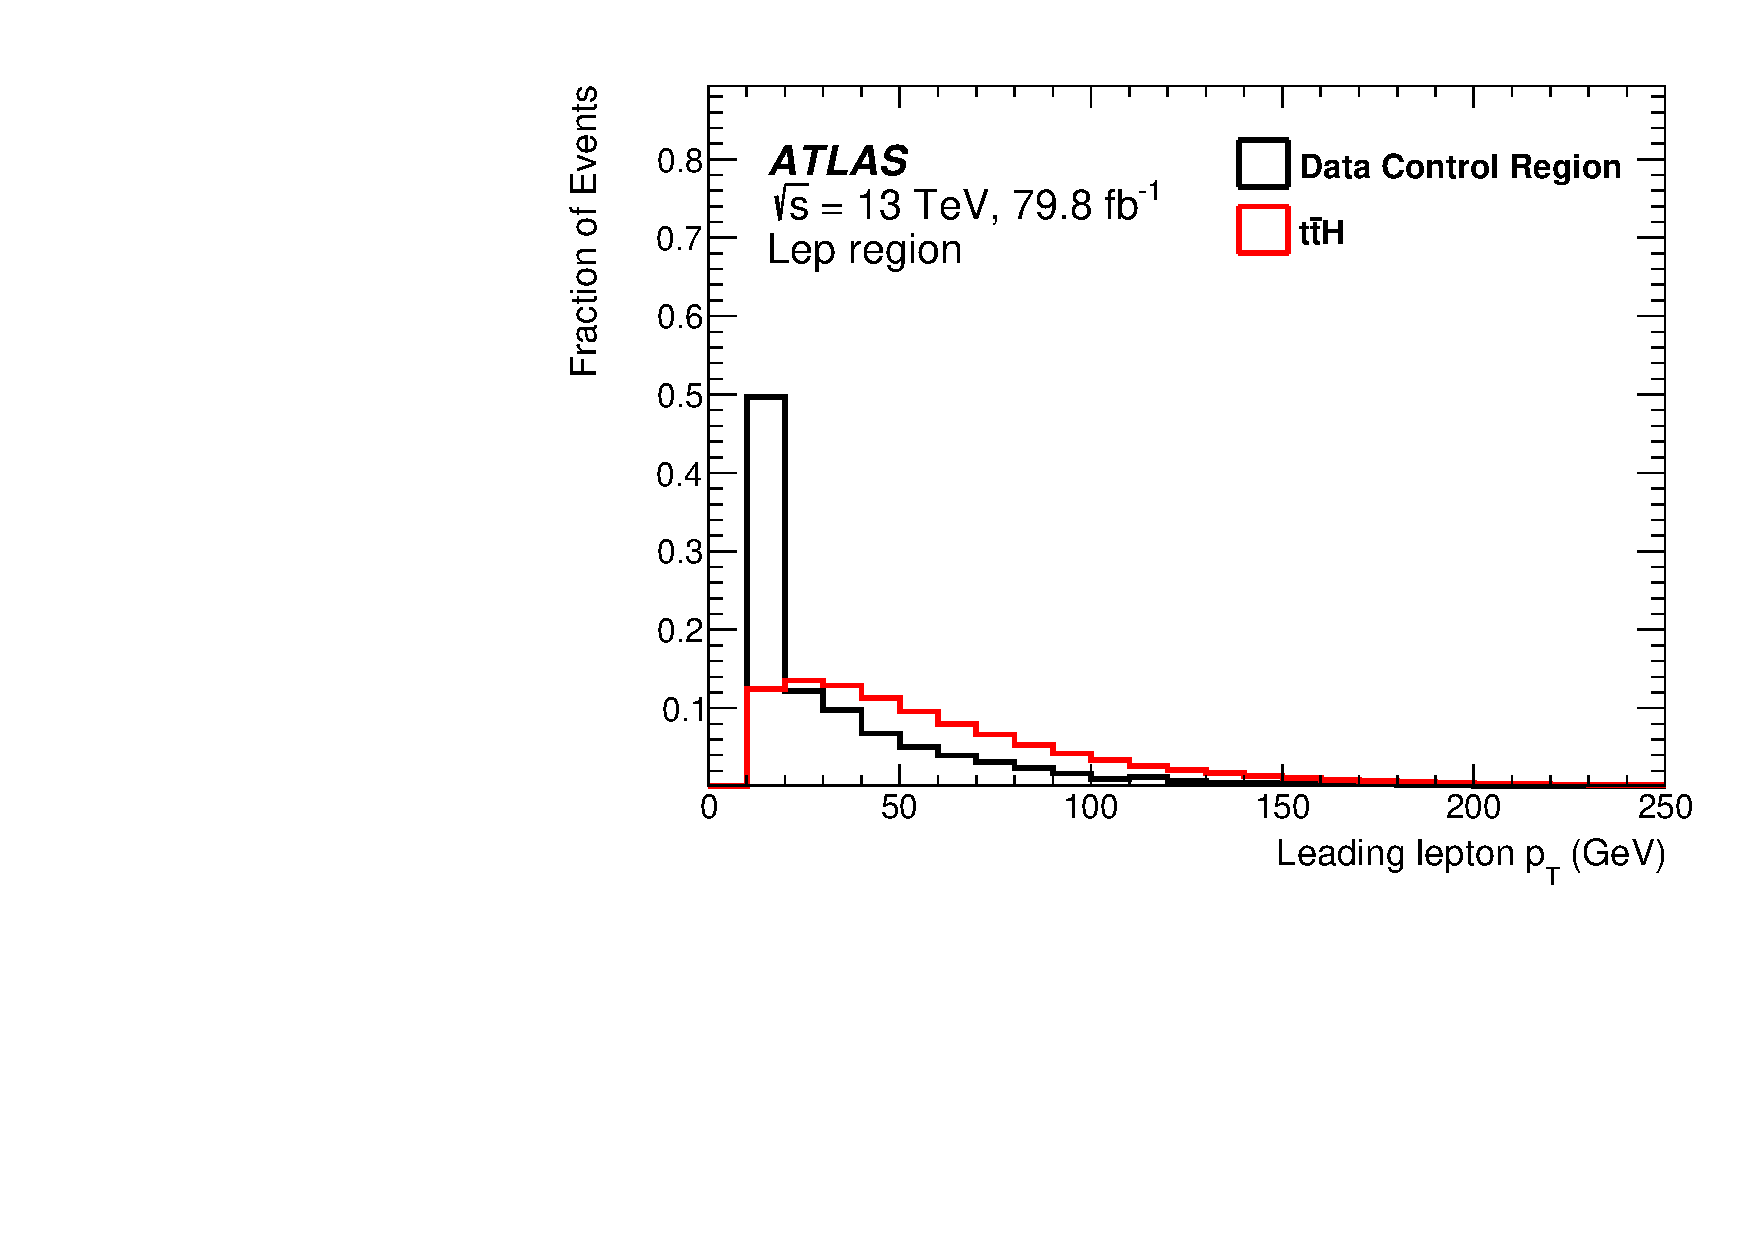
\includegraphics[width=0.31\linewidth]{figures/tthcp_chapter/figaux_11e.pdf}
	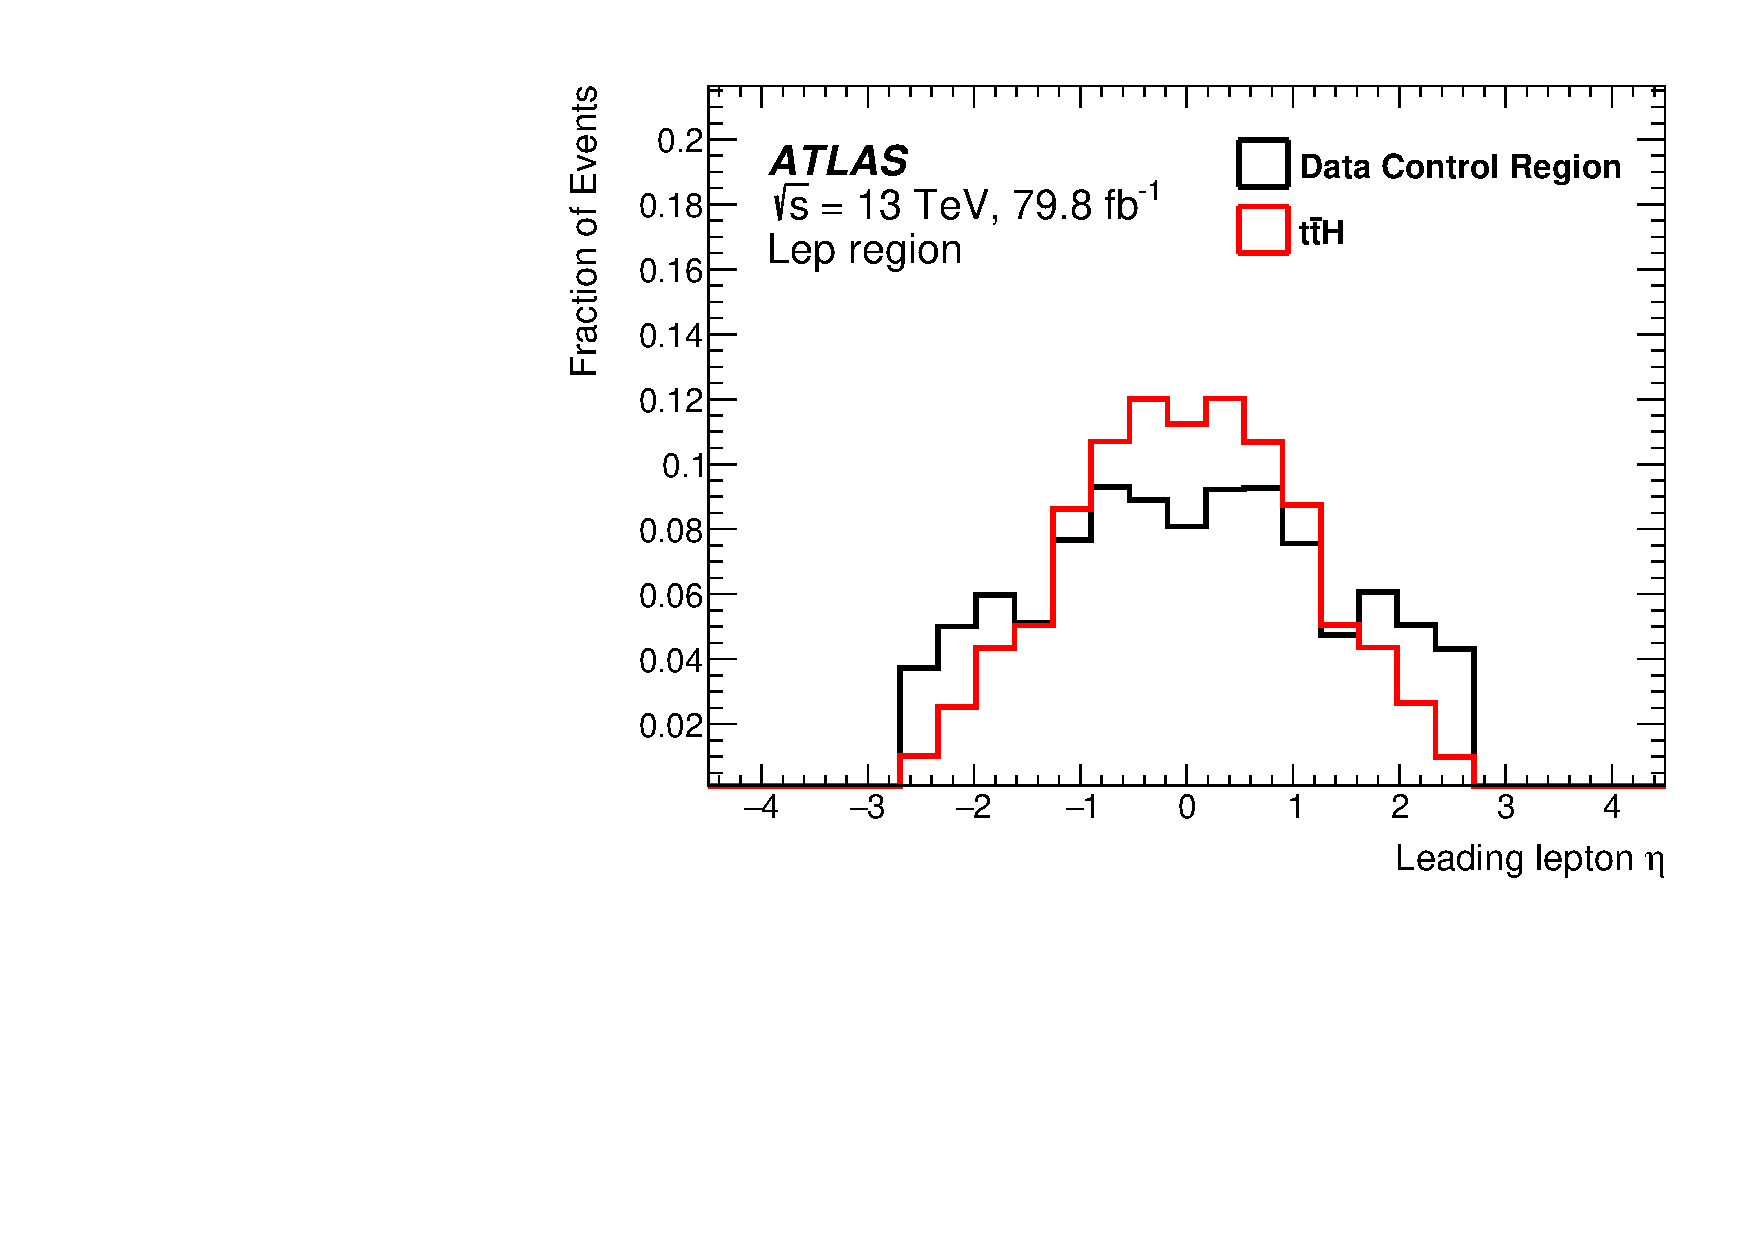
\includegraphics[width=0.31\linewidth]{figures/tthcp_chapter/figaux_11f.pdf}
	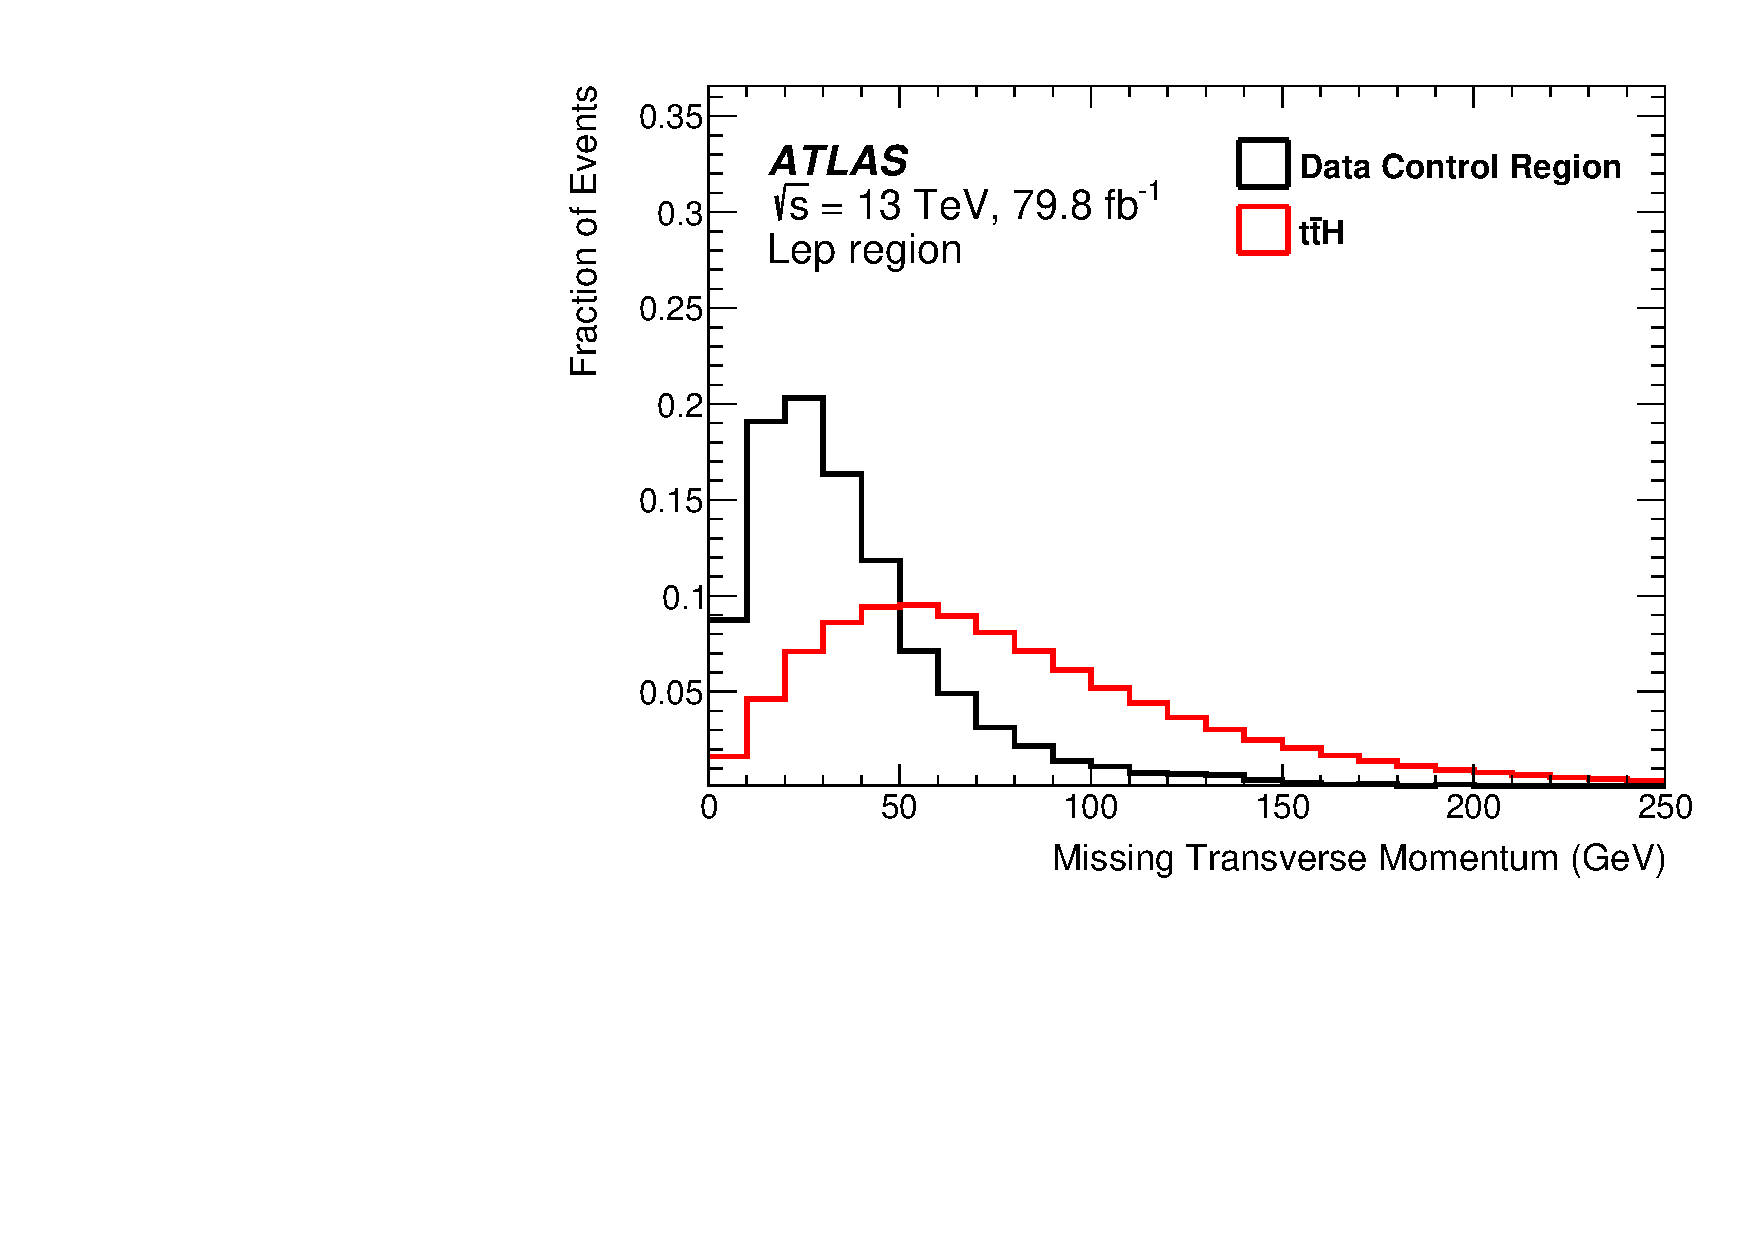
\includegraphics[width=0.31\linewidth]{figures/tthcp_chapter/figaux_11g.pdf}
	\caption{Distributions of training variables for the leptonic background-rejection BDT, trained at 79.8 fb^{-1}. Taken from \ref{cite:HIGG-2018-13}.}
	\label{fig:SBBDTvarslep}
\end{figure}

\ifffalse
\begin{figure}[htbp]
  \centering
        \subfloat[$ttH$ had]{\includegraphics[width=0.3\textwidth]{figures/preselection_and_reconstruction/ttH_had/m_score_wisc.png}}
        \subfloat[$tHjb$ had]{\includegraphics[width=0.3\textwidth]{figures/preselection_and_reconstruction/tHjb_had/m_score_wisc.png}} \\
        \subfloat[$tWH$ had]{\includegraphics[width=0.3\textwidth]{figures/preselection_and_reconstruction/tWH_had/m_score_wisc.png}}
        \subfloat[$ggH$ had]{\includegraphics[width=0.3\textwidth]{figures/preselection_and_reconstruction/ggH_had/m_score_wisc.png}}
  \caption{SB BDT score for $ttH$, $tHjb$, $tWH$ and $ggH$ in the hadronic channel, for various CP mixing scenarios. The open squares show data in the NTI sideband region, giving an approximation of the shape of the continuum background.  }
  \label{fig:moriondhad}
\end{figure}

\begin{figure}[htbp]
  \centering
        \subfloat[$ttH$ lep]{\includegraphics[width=0.3\textwidth]{figures/preselection_and_reconstruction/ttH_lep/m_score_wisc.png}}
        \subfloat[$tHjb$ lep]{\includegraphics[width=0.3\textwidth]{figures/preselection_and_reconstruction/tHjb_lep/m_score_wisc.png}}
        \subfloat[$tWH$ lep]{\includegraphics[width=0.3\textwidth]{figures/preselection_and_reconstruction/tWH_lep/m_score_wisc.png}}
  \caption{SB BDT score for $ttH$, $tHjb$ and $tWH$ in the leptonic channel, for various CP mixing scenarios. The open squares show data in the NTI sideband region, giving an approximation of the shape of the continuum background.  }
  \label{fig:moriondlep}
\end{figure}
\fi

\begin{figure}[htbp]
  \centering
        \subfloat[Hadronic $ttH+tHjb+tWH$]{\includegraphics[width=0.3\textwidth]{figures/categorization_xgb/had-vbls/m_score_wisc.png}}
        \subfloat[Leptonic $ttH+tHjb+tWH$]{\includegraphics[width=0.3\textwidth]{figures/categorization_xgb/lep-vbls/m_score_wisc.png}}
  \caption{SB BDT score for the sum of $ttH$, $tHjb$ and $tWH$, with relative weights according to the predicted cross sections. Shown in (a) for the hadronic channel and (b) for the leptonic channel, for various CP mixing scenarios. The open squares show data in the NTI sideband region, giving an approximation of the shape of the continuum background.  }
  \label{fig:moriondtotal}
\end{figure}


\subsection{CP-Sensitive Observables}

In order to train a BDT to discriminate between CP-even and CP-odd $ttH+tH$, we must plot variables at truth-level and investigate their dependence on $\alpha$. We use the HC model $ttH$ and $tH$ samples with alternative values of $\alpha$ generated using MadGraph5_aMCatNLO, added according to their calculated cross-sections given in table XXX.

From these plots, we observe that the strongest variable is the Higgs boson $p_{T}$ : CP-odd $ttH$ and $tH$ have a much more boosted Higgs than CP-even $ttH$ and $tH$, and are more central in $\eta$. Similarly, the angular separation $\Delta \eta$ between the top and anti-top is much larger in CP-odd $ttH$, while the top and anti-top are more back-to-back in azimuthal angle $\Delta \phi$ in CP-even $ttH$ than in CP-odd $ttH$. In $tHjb$ events, we note that the top $p_{T}$ and $\eta$ also have discriminatory power. The mass of the Higgs + leading top system also offers discriminatory power- for $ttH$ and $tWH$ events it increases with $\alpha$, while for $tHjb$ events it decreases with $\alpha$ .

These variables are shown in Figures XXX through XXX.

\begin{figure}
\end{figure}

\subsection{CPBDT}

Similar to the SBBDT case, two dedicated CPBDTs are trained using XGBoost, one in the hadronic preselection region and one in the leptonic preselection region. An alternative implementation of the BDT is developed using the Toolkit for Multivariate Analysis (TMVA) \ref{cite:TMVA} and is discussed in Appendix \ref{sec:TMVABDT}. Studies performed with the TMVA BDT helped guide the implementation of this BDT, including making the determination that only one dedicated CP-even vs CP-odd BDT was needed (rather than training for multiple $\alpha$ points) and the discovery of several useful high-level variables.

The signal samples are the CP-odd $ttH+tWH+tHjb$, added according to their predicted cross-sections, while the background samples are the CP-even $ttH+tWH+tHjb$. 50\% of the signal and background samples are used for training, 25 \% are used for categorization, and 25\% are used for testing and significance evaluation.

\subsubsection{Hadronic Region} \label{sec:CPBDThad} 

For both the hadronic and leptonic CPBDTs, input variables chosen are:

The training variables used in the hadronic CP BDT training are:
\begin{itemize}
\item $p_{T}$ and $\eta$ of the Higgs candidate
\item $p_{T}$, $\eta$, $\phi$ (with respect to the Higgs candidate), and BDT score of the first and second reconstructed tops. Due to its potential to be composed of fewer than three jets, the second top is referred to as the 'hybrid' top. In the case where no hybrid top is reconstructed, a dummy value is passed to XGBoost.
\item Angles $\Delta\eta$ and $\Delta\phi$ between the top candidates. In the case where no hybrid top is reconstructed, a dummy value is passed to XGBoost.
\item Two-object invariant masses $m_{t1H}$, and $m_{t1hy}$. In the case where no second hybrid top is reconstructed, a dummy value is passed to XGBoost.
\item $H_{T} = \sum_\text{jet j} p^{j}_{T}$
\item The minimum $\Delta$R between a photon and a jet in the event (out of all photon-jet combinations)
\item The second-smallest $\Delta$R between a photon and a jet in the event (out of all photon-jet combinations)
\item Jet multiplicity and $b$-jet multiplicity (77\% working point)
\item Missing $E_{T}$ significance = $E_{T}^\text{miss}/\sqrt{H_{T}}$
\end{itemize}

The XGBoost BDT parameters are optimized by running the training 100 times with hyper-parameters selected according to a Bayesian minimization procedure \cite{skopt}. The integral of the Receiver Operating Curve (ROC AUC) is used as the optimization metric, evaluated on the validation set for each training. The ROC-AUC measures true-positives versus true-negatives, parameterized as a function of classifer threshold cuts: a completely random classifier has a ROC-AUC of 0.5, while a perfect classifier has a ROC-AUC of 1.0 \ref{cite:ROC}. The ROC-AUC for the hadronic CPBDT is 0.7839, while the ROC-AUC for the leptonic BDT is 76.69.

Plots of the CPBDT input variables for the leptonic BDT are shown in figures XXX - XXX, while plots of the CPBDT input variables are shown in figures XXX - XXX.

Plots of the CPBDT output score for both the hadronic and leptonic CPBDT are shown in figures XXX and XXX, while two-dimensional plots of CPBDT score versus SBBDT score for data in both the hadronic and leptonic regions are shown in figure XXX.

\subsection{Poisson Number-Counting Significance}
In order to determine the optimal categorization based on BDT score, two Poisson number-counting significance metrics are used.

In physics analyses such as those discussed in this dissertation, the probability of observing k events in a given region of phase space given an expected number of events $\lambda$ is modeled by a Poisson distribution:

\begin{equation}
P(k, \lambda) = \frac{\lambda^{k}e^{-\lambda}}{k!}
\end{equation}

To determine the compatibility of the observed number of events with a given signal hypothesis H vs the Standard Model, we can define a test statistic called the Poisson Number-Counting Significance:

\begin{flalign}
\begin{aligned}
Z^{2} = -2 ln(\frac{P(S + B, S_{H} + B)}{P(S + B, S + B)}) \\
= 2(S + B) ln(\frac{(S + B)}{(S_{H} + B)} -2(S + B) + 2(S_{H} + B)
\end{aligned}
\end{flalign}

Where S and B are the Standard-Model predicted signal and background and $S_{h1}$ is the predicted signal under hypothesis H.

Thus, we can define the $ttH+tH$ Standard-Model number-counting significance (the significance of observing the amount of $ttH+tWH+tHjb$ in our categories predicted by the Standard Model if in fact the signal process does not exist and the background-only "null hypothesis" is true) as

\begin{align}
Z_{ttH+tH} = \sqrt{2((S+B)\ln(1+S/B)-S)}
\label{eq:ncztth}
\end{align}

and the CP-Odd number-counting significance as:

\begin{align}
Z_{CP}(90) = \sqrt{2(S_e + B)\ln(\frac{S_e+B}{S_o + B}) -2(S_e + B) + 2(S_o + B)}
\label{eq:nczcp}
\end{align}

where $S_{e}$ is the amount of signal expected if $\alpha = 0^{\deg}$ and $S_{o}$ is the amount of signal expected if $\alpha = 90^{\deg}$.

To determine the total significance for either of these metrics across a number of categories, the number-counting significances for each category are added in quadrature.

To estimate the number of continuum background events B in the diphoton mass signal region in each category (that is, $123 GeV < m_{\gamma\gamma} < 127 GeV$), we use a scaling method applied to the NTI data control region in the mass sidebands (that is, $105 GeV < m_{\gamma\gamma} < 123 GeV$ or $127 GeV < m_{\gamma\gamma} < 160 GeV$):

\begin{flalign}
\begin{aligned}
N(TI,signal window) = N(NTI, mass sidebands)\times \frac{N(TI, mass sidebands)}{N(NTI, mass sidebands)} \times \frac{N(NTI, signal window)}{N(NTI, mass sidebands)} \\
= N(NTI, mass sidebands) \times f_{1} \times f_{2}
\end{aligned}
\end{flalign}

Where the scale-factors $f_{1}$ and $f_{2}$ are calculated separately using the hadronic and leptonic preselection regions. We find that the combined scale factor, $f_{1} \times f_{2}$, is 0.013 for the hadronic region and 0.016 for the leptonic region. 

In order to ensure that there is sufficient data to perform a likelihood fit, we require at least 0.8 continuum events (as modelled by scaled NTI sidebands) in the $123 GeV < m_{\gamma\gamma} < 127 GeV$ signal window in each category.

\subsection{2D Categorization}

To perform the categorization, we perform a brute-force scan across many different sets of category boundaries, calculating both $Z_{ttH+tH}$ and $Z_{CP}(90)$ on the validation set. Because the same categorization scheme does not optimize both metrics, a compromise scenario is constructed, for which $Z_{ttH+tH}$ is maximized while $Z_{CP}(90)$ is required to be no more than $0.15\sigma$ less than its maximal determined value. The brute-force scan, and this effect, is shown in figure XXX. The categories selected are given in table XXX. The expected yield and purity in each category is given in figure XXX.

\begin{figure}
\end{figure}

\begin{figure}
\end{figure}

The background-only statistical uncertainty in a given category is given by:

\begin{align}
s = \frac{S}{Z_{ttH+tH}}
\label{eq:statunc}
\end{align}

\begin{figure}
\end{figure}

Using this, we can compare the effects of major systematics to ensure they do not need to be accounted for at the categorization stage. This is shown in table XXX- in all categories, it is clear that the statistical uncertainty dominates.

